% 设置 biblatex 额外选项
% \PassOptionsToPackage{gbpub=false, gbtype=false}{biblatex}

% 载入 SJTUThesis 模版
% \documentclass[degree=doctor, zihao=-4, language=english, review]{sjtuthesis}
% \documentclass[degree=master, zihao=-4]{sjtuthesis}
\documentclass[degree=bachelor, openany, oneside]{sjtuthesis}
% \documentclass[degree=course, language=english, openright, twoside]{sjtuthesis}
% 选项
%   degree=[doctor|master|bachelor|course],     % 必选,学位类型
%   language=[chinese|english],                 % 可选(默认:chinese),论文的主要语言
%   bibstyle=[gb7714-2015|gb7714-2015ay|ieee],  % 可选(默认:gb7714-2015),参考文献样式
%   review,                                     % 可选(默认:关闭),盲审模式

% 所有其它可能用到的包都统一放到这里了,可以根据自己的实际添加或者删除。
\usepackage{sjtuthesis}
\usepackage{multicol}
% 定义图片文件目录与扩展名
\graphicspath{{figure/}}
\DeclareGraphicsExtensions{.pdf,.eps,.png,.jpg,.jpeg}

% 导入参考文献数据库
\addbibresource{bib/thesis.bib}

% 信息录入,必须在导言区进行!
% !TEX root = ../thesis.tex

%TC:ignore

\title{关于深度学习视频流推理任务的通用编程框架的研究}
\author{梁若凡}
\studentid{516030910383}
\supervisor{冷静文 特别副研究员}
% \assisupervisor{某某教授}
\degree{工学学士}
\major{计算机科学与技术}
\department{电子信息与电气工程学院}
\coursename{某某课程}
\date{2020年05月25日}
% \fund{国家 973 项目 (No. 2025CB000000) \\ 国家自然科学基金 (No. 81120250000)}
\keywords{深度学习, 视频流处理,编程框架, 并行优化}

\entitle{A Sample Document for \LaTeX-based SJTU Thesis Template}
\enauthor{Mo Mo}
\ensupervisor{Prof. Mou Mou}
% \enassisupervisor{Prof. Uom Uom}
\endegree{Master of Engineering}
\enmajor{A Very Important Major}
\endepartment{Depart of XXX}
\endate{Dec. 17th, 2014}
% \enfund{National Basic Research Program of China (Grant No. 2025CB000000) \\
%   National Natural Science Foundation of China (Grant No. 81120250000)}
\enkeywords{SJTU, master thesis, XeTeX/LaTeX template}

%TC:endignore


% 自定义项目标签名称
% \sjtuSetLabel{
%   listfigure = {图\quad 录},
%   listtable  = {表\quad 录}
% }

\begin{document}

% 无编号内容:中英文论文封面、授权页
\maketitle
% \makeDeclareOriginality[pdf/originality.pdf]
% \makeDeclareAuthorization

% 使用罗马数字对前言编号
\frontmatter

% 摘要
% !TEX root = ../thesis.tex

\begin{abstract}
深度学习相关软、硬技术在近年来飞速发展使得对视频流内容进行连续的智能分析与推理成为了可能。准确、高效的智能视频分析、理解对未来生产生活的方方面面都有着及其重要的应用价值。然而深度学习相关的视频流处理往往有着较为复杂的计算流程,十分依赖不同模块/代码库的协同计算,有一定的开发门槛与上手难度。此外,深度学习方法目前相比仍然需要数倍于传统视觉算法的计算开销,这种高计算开销也导致了深度学习视频处理任务难以在一般硬件上取得较高的帧率。
% 深度学习技术近年来在计算机视觉领域取得了显著的成就,其相关的计算机视觉算法已经逐步应用到了各类现实应用或生产过程之中。视觉算法性能以及硬件算力的不断提升使得对视频流内容进行连续的智能分析与推理成为了可能。
\end{abstract}

\begin{enabstract}
  Shanghai Jiao Tong University (SJTU) is a key university in China. SJTU was
  founded in 1896. It is one of the oldest universities in China. The University
  has nurtured large numbers of outstanding figures include JIANG Zemin, DING
  Guangen, QIAN Xuesen, Wu Wenjun, WANG An, etc.

  SJTU has beautiful campuses, Bao Zhaolong Library, Various laboratories. It
  has been actively involved in international academic exchange programs. It is
  the center of CERNet in east China region, through computer networks, SJTU has
  faster and closer connection with the world.
\end{enabstract}


% 目录、插图目录、表格目录
\tableofcontents
\listoffigures
% \listoftables
\listofalgorithms

% 主要符号、缩略词对照表
% \input{tex/nomenclature}

% 使用阿拉伯数字对正文编号
\mainmatter

% 正文内容
% !TEX root = ../thesis.tex

\chapter{绪论}

\section{基于深度学习的计算机视觉技术} \label{intro_dl}
以深度学习为代表的机器学习算法近年来在学术研究与生产应用的各个领域中备受关注。凭借其较强的特征与知识表征能力,飞速发展的深度学习算法逐渐在计算机视觉,自然语言处理,语音识别等识别与感知挑战中取得接近甚至超越人类的表现\cite{he2016deep, hochreiter1997long, hinton2012deep}。%(加Cite呀)
深度学习模型往往依赖大规模数据集通过反向传播算法训练、优化得到的模型的权重参数.输入数据与这些权重参数进行一系列运算最终输出各类检测或识别的推理结果\cite{lecun2015deep}。无论是前向推理还是反向传播训练都需要处理大量的矩阵计算,因而深度学习的发展也离不开相关系统框架以及硬件架构的针对性优化与发展。\par

深度学习算法源于多层感知机模型(Multi-Layer Perceptron,MLP)的不断改进与优化。MLP是一种由全连接层(权重矩阵)和非线性激活函数共同构成的浅层神经网络。随着相关理论以及计算机算力的发展,神经网络的层数逐渐变深,不同类型的网络连接层、网络结构相继被提出。这一系列的发展使得深度学习模型有了更强的信息提取能力,在性能上逐步超越传统的人工设计的专家系统。\par
在计算机视觉领域,深度学习模型主要以卷积神经网络(Convolutional Neural Network, CNN)的形式的存在。CNN借鉴了传统数字图像处理中卷积操作的概念,它权重共享以及平移不变的特性一方面大大减少了深层神经网络的参数,另一方面体现了CNN算法对不同图像特征提取的普遍适应性。
% emmm 要不要加个公式意思一下呢。。。 算了。。。
LeNet\cite{lecun1990handwritten}是CNN的早期代表模型,它被成功应用到了手写数字识别任务上。2012年的AlexNet\cite{krizhevsky2012imagenet}使用了在GPU上实现的深层卷积神经网络结构,在当年的大规模视觉识别挑战(ImageNet\cite{deng2009imagenet})中取得了突破性的精度提升。AlexNet的出色表现也直接催生了后续深度学习技术的井喷式发展,从VGG\cite{simonyan2014very},Inception\cite{carranza2017going},到ResNet\cite{he2016deep},再到如今的网络架构搜索(Neural Architecture Search, NAS\cite{tan2019efficientnet}),CNN模型在精度和性能上都在不断地提升。如今各类视觉任务往往会利用这些出色的网络架构作为骨架来提取图像中的特征知识。\par
在具体视觉应用领域,计算机视觉也在近年来做到了从最初图像分类,人脸识别到目标检测,关键点检测,图像分割,图像生成等应用的全面发展。以目标检测为例,最开始R-CNN\cite{girshick2014rich}提出了区域推荐(Region Proposal)的方式完成目标检测。后来又有如Faster R-CNN\cite{ren2015faster},Mask RCNN\cite{he2017mask}等算法将以Region Proposal为主的检测方式逐步优化,不断提高模型的精度与运行效率。同时也有以YOLO为代表的一系列检测算法对检测任务直接进行端对端的神经网络训练,模型的精简使得这种方法可以实现目标检测的实时推理。这些日益成熟的深度学习计算机视觉技术也为无人驾驶,智能机器人,智慧城市等新兴研究方向提供了必要的技术支持,会在以后的生产生活中发挥重要的作用。\par
如今深度学习算法在各个领域中已取得了初步的成效,当前深度学习技术发展主要关注在模型的压缩、剪枝、量化方法,自动化的机器学习算法开发(AutoML),深度神经网络黑盒模型的可解释性与安全性分析等方面,进一步提高深度学习模型的计算性能,开发效率以及应用可靠性。

\section{视频流处理模型与流程}\label{intro_vp}
从广义上来讲,视频流处理是对视频流信息进行一系列的数字信号处理以满足特定应用场景对视频资源的需求。传统意义上的视频处理任务包括视频压缩与编码,视频超分辨,视频插帧,视频内容分析等多个方面。数字图像处理技术的长期发展已经使一些传统视频处理任务如编码、压缩、降噪、防抖等有了较好的解决方案。而本文讨论的视频流处理主要是指对视频流内容的分析与检测,这类视频分析任务当前的发展也是与\ref{intro_dl}中讨论的基于深度学习的计算机视觉算法有着密切的关系。\par
视频分析任务又可以被细分为目标检测与追踪,动作感应,姿态识别,图像分割,图像/视频增强等具体的应用类型。% 讲一下这些复杂CNN模型吧
这些在视频理解任务中使用到的深度视觉算法往往会由一些神经网络模型组合而成。首先,原始输入图像数据会通过一些典型的预训练CNN网络(如VGG\cite{simonyan2014very}, ResNet\cite{he2016deep}, MobileNet\cite{howard2017mobilenets}等)提取出高维特征信息,然后,这些特征信息将会作为特定任务算法模型的输入进行接下来的机器学习分类或回归任务。这种算法模式常见于目标检测,图像分割以及图像增强等应用任务中,代表模型有R-CNN\cite{he2017mask}系列,DeepLab\cite{chen2017deeplab}系列,以及其他解码-编码(Encoder-Decoder)模式的图像生成模型。另一种常见的应用场景是直接的多模型应用,比如在一些如人脸,人体的关键点的检测任务上。为了保证模型的精度,这类任务往往需要先运行一个目标检测的神经网络来获得目标相关的检测边框,利用获得的检测边框对原始图片输出进行进行再次的剪裁、缩放、旋转等操作,然后将处理得到的图片送入关键点检测的回归预测模型中,最终获得检测结果\cite{fang2017rmpe,zhang2016joint}。% e.g. alpha pose, MTCNN
除此之外,更为综合的视频分析可能需要对同一视频源进行多类型的视频识别,检测与理解任务。如CMU的开源项目OpenPose\cite{cao2018openpose},有三个相对独立的神经网络算法分支同时对视频中的人体骨架,手部姿态以及人脸关键点进行检测与估计。\par
\begin{figure}[!htp]
    \centering
    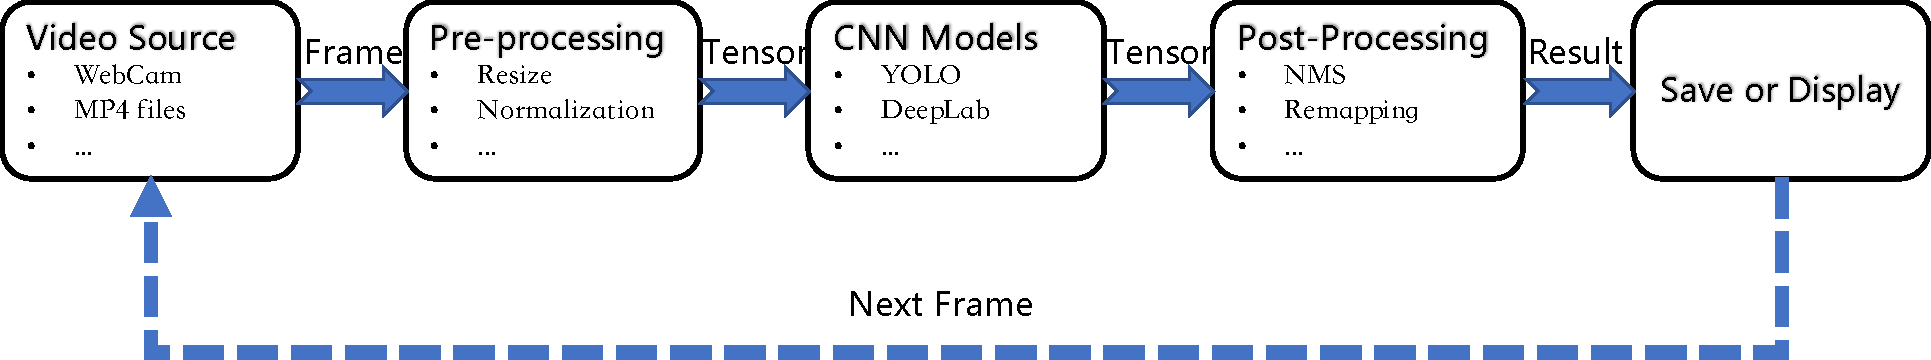
\includegraphics[width=\textwidth]{figure/video_proc_flow.pdf}
    \bicaption{深度学习下视频流处理的一般流程}{Genral process of deep learning based video processing workflow}
    \label{fig:video_proc_flow}
\end{figure}
在深度学习技术的背景下,这些视频分析任务虽然会使用到不同的机器学习算法的组合,但是也存在着许多共通的处理流程。% (emmm,可以考虑加一个流程示意图)
一般情况下,视频流的处理可以看作是在连续的视频帧上做单张图像的视觉计算。因此,视频处理通常由视频流的读取,视频帧的预处理,视觉算法模型(CNN)的运行,算法推理结果的后处理,以及结果的输出与展示这几部分共同来构成,如图\ref{fig:video_proc_flow}所示。当然,对于具体的现实任务来说每一个处理步骤中可能还存在一系列的子步骤,最终会使得整个处理流程的可视化表示变成一个较为复杂的有向无环图(Directed Acyclic Graph,DAG)\footnote{这里不考虑如图\ref{fig:video_proc_flow}中前后帧之间的连接。}。 本文接下来要讨论的视频流处理的优化工作也是基于对视频处理的这种理解与抽象。\par

\section{视频流处理的优化策略}\label{intro_opt}
在\ref{intro_vp}中讨论的视频流处理过程可以进行多层面的优化。从底层硬件到系统运行框架再到算法层面,都有着相应的优化工作。一些相关优化工作也会在第\ref{related_work}章做进一步的讨论。因此本部分仅对相关优化策略做简单介绍:\par

\subsection{针对整体处理流程的系统优化。}\label{sub:sys_opt}
对于像图\ref{fig:video_proc_flow}所示的视频处理过程,由于其存在多阶、相互依赖的连续数据处理的特点,视频处理算法的部署可以参考现代CPU流水线式的处理逻辑,通过多级流水线的模式来部分掩藏处理流程中瓶颈模块的计算耗时。另一方面,对于较复杂DAG连接的视频处理任务,其任务本身就存在一定的并行度,可同时对多个模块并行处理。
\subsection{针对视频特性的视觉算法优化}\label{sub:algo_opt}
现有的深度学习视频分析处理算法多数是直接对视频中的每一帧单独运行原本应用在图像上的视觉算法模型,较少考虑视频帧与帧之间连贯性的特点做算法上的专门优化,从而减少算法在处理过程中的冗余或者非必要计算。在利用视频信息的连贯性上,可引入视频光流估计方法,将前帧的计算结果更快速地传递给后一帧,如Zhu et al.提出的DFF(Deep Feature Flow)模型\cite{zhu2017deep};也可以利用视频编码如H.264\cite{tourapis2003fast}中包含的运动向量(Motion Vector)信息,来对视频关键帧进行选择性检测与传播,如Mao et al.提出的MobiEye\cite{mao2019mobieye};
还可以单纯利用短时间内物体的位移量较小的特点,直接利用上一帧的检测结果,进行接下来的细粒度检测,如Google 的人手追踪模型\cite{mediapipe_hand}。此外,也可利用视频帧的上下文信息来提升视频单帧的检测精度\cite{zhu2017flow}。
\subsection{针对神经网络推理的加速优化}\label{sub:infer_opt}
整个深度学习视频处理流程中的速度瓶颈往往是在神经网络模型的推理步骤上,如\ref{intro_dl}中所说,深度神经网络的推理通常需要进行大量的矩阵计算,有数倍于传统计算处理步骤的时间开销。因此在近年来关于神经网络的压缩,剪枝,量化的研究收到了极大的关注。这些技术从不同的角度对深度神经网络模型精简,在保持模型精度的条件下,尽可能减少模型所需计算资源,提升模型运行速度。此外也有专门针对神经网络推理运算的系统层面的优化加速,比如对需要推理的网络模型进行重编译,对满足特定条件的计算步骤进行融合,从而降低相应算子的调用开销,并优化内存空间的使用。

\subsection{针对模型计算特性的硬件优化}\label{sub:HW_opt}
日渐成熟的深度学习算法的使用也促进了相关硬件平台的发展。深度神经网络所需要进行的矩阵运算对并行计算有着天然的适应性。各大厂商生产的GPU,TPU,VPU等异构芯片在处理这类简单多数据计算时相比传统CPU芯片有着明显的优势。Nvidia在近年来着重发展其GPU产品的AI计算能力,在Volta架构后,为其GPU添加了专门的Tensor Core计算核心来提高其在大量矩阵运算上的处理性能;Google在TPU\cite{jouppi2017datacenter}(Tensor Processing Unit)架构中引入了由大量矩阵乘加器构成的脉动阵列(Systolic Array)结构,来提高矩阵运算的吞吐量;Intel也有推出其集成DSP,VLIW,GPU等特性的混合架构VPU\cite{moloney2014myriad}(Vision Processing Unit),来为移动或边缘设备提供视觉相关AI加速计算的能力。\par~\par

本研究期望对具有一般性的基于深度学习的视频处理任务进行部署与性能上的优化,并通过一种通用框架的形式实现。基于这样的研究目标,我们提出了Accel-Video Pipe (简称AVPipe)这一针对智能视频流处理的编程框架。我们在接下来的框架设计与优化的过程中会主要关注\ref{sub:sys_opt}中介绍的视频流处理在系统层面的优化,同时我们的框架会对现有的神经网络推理优化引擎(\ref{sub:infer_opt})以及相应的计算硬件(\ref{sub:HW_opt})提供充分的支持。对于\ref{sub:algo_opt}中的算法层面优化,由于这类有较强的任务相关性,缺少通用性,故在本框架中不做深入,但用户仍可以通过AVPipe实现相应处理任务的算法优化。

\section{论文的主要内容与章节安排}
本论文大致分为五章展开。在接下来的第二章中,我们将对与本文介绍的视频处理相关的已有优化工作进行介绍,并在其中说明现有相关工作的不足以及可借鉴之处。然后在第三章中,我们将总结现有深度学习相关视频处理任务在实际生产应用中的应用需求以及可能存在的问题,并依此来明确我们的研究动机以及研究目标。
在第四章中,我们将详细介绍我们提出并实现的视频流处理编程框架Accel-Video Pipe,这其中包括AVPipe框架的设计逻辑,主体结构,以及它的自动化部署与优化工具。最后,在第五章中,我们将通过几个示例视频项目的开发,以及性能分析对比,来说明本框架在实际应用过程中的有效性。
% !TEX root = ../thesis.tex

\chapter{相关工作}

\section{视频流处理框架}

\section{深度学习推理引擎}

\section{多阶段有依赖任务的调度与划分}

\section{本章小结}
% !TEX root = ../thesis.tex

\chapter{背景和动机}
在这一章,我们会对深度学习背景下视频流处理的实际应用需求以及问题做总结。在此基础上,我们会列出对AVPipe设计的期望与目标。
\section{视频流处理的应用需求}\label{ch3:req}
随着人工智能的发展,不论在生产实践中还是在生活娱乐中,我们都期望人工智能技术能够给现有的应用带来创新。计算机视觉是应用人工智能最主要的领域之一,这之中对视频流的智能分析与推理可以说是许多智能视觉算法的主要现实应用形式。在生产实践中,无人驾驶、智能机器人等技术对智能视频流的推理分析有着直接的技术依赖,智能工厂、智慧城市的建设也需要利用视频的视觉分析来提高管理效率,来实现自动化管理。在生活娱乐中,智能视频处理可以为用户内容创作提供便捷,近年来在智能手机上兴起的视频增强、现实增强功能,如iPhone的Animoji\footnote{\url{https://support.apple.com/en-us/HT208190}}功能,需要智能视频处理及时的支持;
视频内容创作分享平台如抖音\footnote{\url{https://www.tiktok.com/}}、哔哩哔哩\footnote{\url{https://www.bilibili.com/}}等都提供了诸如智能抠图(图像分割),人物识别等功能;高效,准确的视频处理也可以被应用在游戏创作中,为玩家带来玩法上的创新。\par

\section{视频流处理的现存问题}\label{ch3:problems}
针对\ref{ch3:req}中提到的关于视频流处理的应用需求,我们也通过相关产品的实际使用以及一般视频流处理应用的开发实践,总结得出了现在视频流处理的应用与开发中存在的一些问题:\par
% \begin{enumerate}
% \item
\textbf{开发与部署难度大。}深度学习相关视频流处理应用的开发流程一般都是先利用Python环境下的各类机器学习框架(如TensorFlow, PyTorch等)对处理算法做验证与测试,然后再将处理打包或利用其他语言重写。考虑到计算的高效性、代码的安全性以及部署的通用性,一般会将验证通过的视觉处理算法用C/C++语言进行重写。C/C++语言中并没有类似Python中NumPy\cite{oliphant2006guide}的通用科学计算库可以无缝应用在处理流程的各个步骤中,开发人员需要手动完成数据类型以及数据布局在不同计算库之间的转换,这一问题在处理神经网络所涉及的高维张量数据时表现得尤为明显。此外,不同计算库采用的截然不同的代码规范以及调用接口也进一步提高了C/C++语言下视频流处理应用的开发难度。\par
% \item 
\textbf{缺乏针对性优化。}有关视频流处理的优化在本文\ref{intro_opt}中有进行介绍。完善与成熟的相关算法框架的一般都会提供一些示例程序供用户进行学习或使用,如OpenCV中有关DNN的示例\footnote{\url{https://github.com/opencv/opencv/tree/master/samples/dnn}},TensorFlow中有关移动部署的示例\footnote{\url{https://www.tensorflow.org/lite/models/}}。我们尝试在个人设备%\footnote{Intel i5-8210Y处理器的MacBook Air笔记本和Qualcomm 835处理器的Sony XZ1智能手机}
上编译运行OpenCV的目标检测示例以及TensorFlow的人体姿态估计示例,这两者的实际表现并不出色。实际处理帧率远低于可以流畅实时处理的期望。
观察开源代码可知,OpenCV的示例虽提供了简单多线程的运行优化,但其并没有在深度神经网络的推理上提供充分的加速优化;TensorFlow的姿态估计示例则没有在代码中提供充分的非神经网络推理部分的优化,整个处理过程都在单线中进行。与其他将数据传回云端进行处理的人工智能应用(如推荐系统和语音识别)不同的是,视频流处理的数据传输量大,对实时性的要求也相对较高,一般倾向在本地完成大部分计算。这也侧面说明了对视频流处理进行优化的必要性。
% \item 
% \end{enumerate}

\section{研究动机与目标}\label{moti_obj}
以上介绍的基于深度学习的视频流处理应用中所存在的需求与问题促使了我们开展有关视频流处理优化的研究。我们期望提供一种编程模型或框架在解决以上提及问题的同时,满足实际生产的需求。具体来说,我们所提出的框架需要实现以下目标:
\begin{enumerate}
    \item 较完整的视频流处理开发框架,支持视频流处理每一步骤在框架内的实现;
    \item 较为丰富的平台与硬件支持(如主流桌面与移动系统下的多种CPU,GPU);
    \item 提供能够轻松上手的简单直接的开发流程;
    \item 对主流神经网络推理引擎提供统一的支持与封装;
    \item 提供自动化工具对处理流程图进行代码生成生成与运行优化;
    \item 提供性能分析以及可视化展示工具来指导对处理流程的优化。
\end{enumerate}\par~\par
为尽可能地实现以上目标,我们提出并实现了Accel-Video Pipe\footnote{\url{https://github.com/nexuslrf/Accel-Video-Pipe}}这一针对深度学习视频流处理的C++编程框架。我们期望AVPipe的框架能够满足实际视频流处理任务的开发需求。

\section{本章小结}
本章针对实际视频流处理应用中存在的需求与问题做了简单的介绍,分析了视频流处理在生产实践与生活娱乐中的应用前景,也指出了现有应用在开发部署以及运行优化上存在的不足之处。
这些需求与不足也直接引出了本文的研究动机与研究目标——构建一个更为友好,更为高效的C++编程框架AVPipe。在接下来的章节中,我们会对AVPipe的设计与实践做更详细的介绍。
% !TEX root = ../thesis.tex

\chapter{AVPipe视频流处理框架的设计与实现}
为了解决在\ref{moti_obj}中所述的目标,我们设计了Accel-Video Pipe(AVPipe),一套模块化的对基于DAG计算图的视频流处理提供开发便捷以及加速优化的编程框架。在这一章中,我们将具体介绍AVPipe的设计逻辑与框架结构。

\section{AVPipe的设计逻辑}
% 先讲逻辑抽象:
%   以 数据流 ,数据处理的分离。由管道将数据与不同处理模块相连接。
% 再讲各部分是如何设计的 
针对视频流处理任务在多阶段有依赖的较复杂计算流程,我们需要使AVPipe编程框架能够对整个智能视频处理流程进行合理的抽象。\par
视频流处理中,数据是不断地由起始节点(source),经过一步步的计算流向汇聚节点(sink)的。这一过程中,数据是在整个计算流程中持续变化的,此外,这些产生的数据也存在着时序上的依赖关系。另一方面,处理流程图中的每一个计算节点所承担的计算任务是固定的。为了对计算流程图进行管理与优化,所有计算模块需要有通过一套简单的、统一的类(class)或结构(struct)来进行封装。\par
基于以上两方面的考虑,我们将AVPipe中的数据与数据处理单元分离开来,分别抽象为StreamPacket和PipeProcessor。为实现数据与数据处理单元之间的交互,我们又建立了对数据流的抽象Stream。数据流(Stream)将不同数据处理单元(PipeProcessor)连接成一个整体,为数据(StreamPacket)提供了流动的载体与指引,使得数据可以有序地、高效地流向各个处理单元。 对数据,数据流以及数据处理单元的抽象是AVPipe框架的主要设计逻辑,图\ref{fig:base_struct}直观展示了这三者在AVPipe中的关系。接下来我们会逐一介绍这三部分的具体设计。
\begin{figure}[htp]
    \centering
    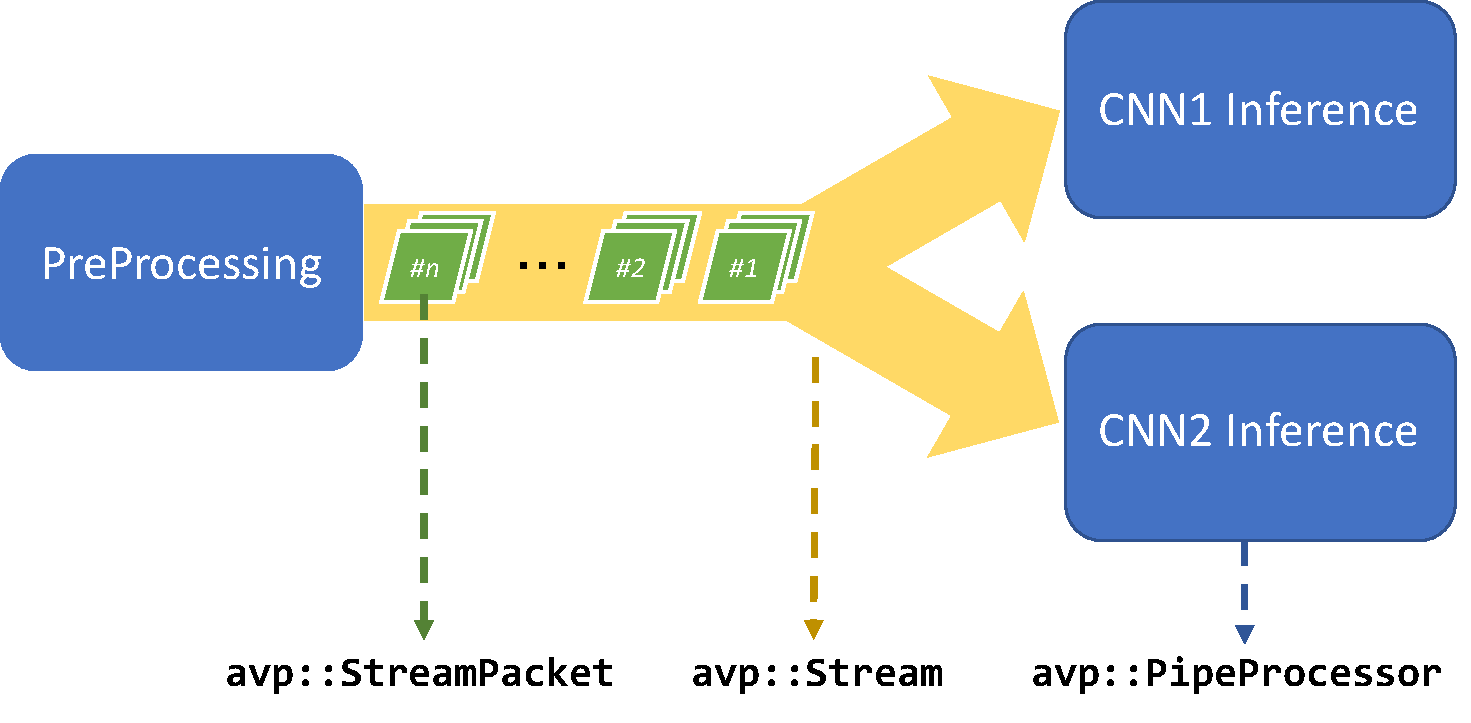
\includegraphics[width=0.8\textwidth]{figure/avp_base_struct.pdf}
    \caption{AVPipe基本抽象之间的关系}
    \label{fig:base_struct}
\end{figure}
\subsection{数据包StreamPacket}
StreamPacket中包含了视频流处理流程中的待处理数据。每个StreamPacket只表示单一类型的数据(如图片,矩阵或张量等)。
为了保证数据的同步与时序,每个StreamPacket都有一个时间戳(timestamp)来记录自己的创建时间步,同一时间步的所有StreamPacket需要在同一处理流程周期中完成。
考虑到某些数据处理步骤可能会在同一时间步中产生多个处理结果,数据在StreamPacket中需要以列表的形式来进行维护。某些数据处理过程也可能会由于没有满足条件而产生空的数据包,空数据包作为作为处理流程中的正常产物,StreamPacket仍然需要对其提供必要的处理逻辑。此外,由于整个AVPipe的数据处理是围绕着StreamPacket来进行的,当整个处理流程结束时,需要依赖StreamPacket的传播来告知每个数据单元来停止运行,因此除了空数据包外,StreamPacket还需提供携带结束信息的终止数据包。
\subsection{数据流Stream}\label{ch4:design_stream}
Stream是StreamPacket的载体,其主体需要存在一个队列结构来有序存取StreamPacket。另一方面,Stream又有着连接PipeProcessor的作用,由于同一个人数据可能会被多个步骤利用,因此同一个Stream可能会同时连接多个PipeProcessor(如图\ref{fig:base_struct})。考虑到多个PipeProcessor可能会多线程同时运行,Stream需要为此提供一定的同步与阻塞机制,以免数据的错位与误读。
当数据包完成在PipeProcessor被使用并完成处理时,PipeProcessor会向Stream发送该数据包的释放请求,Stream要能判断该数据包是否被所连接的所有PipeProcessor全部使用,当且仅当所有PipeProcessor都使用了该数据包后,数据包才会从Stream中安全释放。
有时候,由于数据生产速度会超过数据消费速度,数据包StreamPacket会不断地积累在Stream中而不能及时处理,最终导致大量内存的不必要消耗。为此,Stream还需要提供一个长度或容量的限制,结合阻塞机制来防止数据包的聚积。

\subsection{数据处理单元PipeProcessor}\label{ch4:design_proc}
PipeProcessor是对视频流处理中各个计算步骤的抽象。PipeProcessor从其连接的输入Stream中拿到数据进行处理,将计算结果放入输出Stream中。PipeProcessor根据根据其输入输出的方式不同,可以分为三类:
\begin{enumerate}
    \item 数据处理型(Process):既有输入数据,也有输出数据。视频流处理中的绝大多数多数处理模块的属于这一形式;
    \item 数据起源型(Source):只有输出数据。主要用于获取或产生数据源(如视频摄像头的捕捉或视频文件的读取)供接下来的处理使用;由于Source节点为每一次处理的起点,当视频处理任务结束时,需要由其产生终止数据包来传播给其他所有计算节点。
    \item 数据汇聚型(Sink):只有输入数据。主要用于汇集视频处理的结果,用以保存或窗口展示。当所有的Sink节点都收到终止数据包时,这意味着所有计算节点都收到了终止信号,整个视频处理流程就会停止运行。
\end{enumerate}
流处理中的不同处理模块都是对PipeProcessor的继承与实现。不同模块可以定义自己所需的变量或内存,其实际计算则是通过重载PipeProcessor中的运行接口(\texttt{run})来实现的,在这个运行接口中只需要定义处理相关的计算即可。对于运行的前的准备,输入数据的检查,时间戳的校对则是由PipeProcessor内不另一个接口来实现的(\texttt{process}),\texttt{process}要能检查输入的有效性。当输入为空数据包时,\texttt{process}在默认情况\footnote{部分输入数据为空时,数据处理逻辑也有可能产生非空的输出。如对检测结果的在检测帧上渲染时,检测结果可能为空。}下会直接返回空的输出数据,而不调用\texttt{run}接口。\texttt{process}对终止数据包也会有类似的处理,不再赘述。总之,在实际使用中,我们不能直接调用\texttt{run}的接口,
而是通过调用对\texttt{run}再次封装的\texttt{process}接口。这样的设计一方面可以提高代码运行的可靠性,另一方面可以简化不同模块计算流程的实现。

\section{AVPipe的框架实现}
在介绍了AVPipe主体的设计逻辑后,我们将在本小节关注框架实现中存在的需要特别考虑的内容,同样围绕着数据包,数据流以及数据处理单元这三大部分进行展开。
% 讲 Mat 与 Tensor的 整合
\subsection{StreamPacket中数据格式的整合}
针对\ref{ch3:problems}中提到的数据格式在不同处理步骤中的不能不统一使用的问题,我们期望StreamPacket的封装能够在这方面带来改善。对视频流处理这一类任务来说,我们可以将处理流程中可能涉及到处理数据的格式进行总结。通过调研不同视频流处理任务发现,所涉及的数据处理主要包含两种数据格式:(1)图像的矩阵数据,数据主要以OpenCV的Mat格式来参与传统的数字图像处理运算,如图像的裁剪,缩放,仿射变化等,但是Mat数据有维度的限制,如\ref{ch2:framewk}中所说,它不能很好地处理高维张量数据;(2)机器学习相关的张量数据,张量数据主要用于神经网络的计算以及相关的后处理操作中,张量数据在各个深度学习推理引擎中的表示不尽相同,对高维张量的操作难易程度也不尽相同。通过以上分析,我们可以确定的是StreamPacket需要同时对图像矩阵以及高维张量提供良好的支持,接下来我们要考虑具体实现实现方式。\par

首先,在关于图像矩阵的处理上,OpenCV是受业界普遍认可的通用数字图像处理库。因此,在StreamPacket中的数据提供直接的\texttt{cv::Mat}形式的数据存储是对传统数字图像处理操作最友好的支持。
再来看对高维张量的处理。由于这方面的需求是在近些年由机器学习技术的快速发展而兴起的,这使得目前在C/C++语言下没有一个像Python中NumPy那样的,开发完善的,普遍使用的针对高维数据的科学计算库,从而导致不同的机器学习框架会各自为阵,开发仅供本框架使用的数据格式以及数据处理方式,如TVM所使用的DLPack\cite{dlpack}库,PyTorch所使用的ATen库。通过实际使用和测试发现,PyTorch/Caffe2所使用的ATen张量库有最为完善的张量定义以及操作算子,其类似Python的数据操作与丰富的开发文档也带来了出色的使用体验。我们也因此将ATen库中的张量格式\texttt{at::Tensor}做为AVPipe主要支持的张量格式。\par

通过以上分析,我们确立了对\texttt{cv::Mat}以及\texttt{at::Tensor}这两种数据格式的支持,我们现在开始考虑如何对这两部分在StreamPacket中进行有机结合。考虑到OpenCV与LibTorch都是提供预编译的开源库,我们并不打算对这两个库的底层代码进行修改以实现操作的互通,这在工程难度以及通用性上都不可行。于是我们考虑在StreamPacket中同时保留\texttt{Mat}和\texttt{Tensor}的数据队列。通常情况下,一个Stream对应的StreamPacket都是同一个类型的,也就是说,\texttt{Mat}和\texttt{Tensor}两者中一般只有一个保存有待处理数据。PipeProcessor在生成数据时,也会规定数据将在StreamPacket中以哪种方式保存,这使得StreamPacket在管理内部数据时只需关注它所对应形式的数据。
此外,我们也在StreamPacket的内部,通过内存指针引用的方式,提供了\texttt{Mat}和\texttt{Tensor}相互类型转换的方法,为不同应用场景提供便利。

% 同步以及其他特殊情况的考虑
\subsection{Stream中数据的同步与管理}
在\ref{ch4:design_stream}中,我们介绍了Stream的设计逻辑。在这一部分里,我们主要说明在Stream实现过程中要考虑的关键点。由于Stream本质是存放AVPipe数据包的一个队列,因此Stream直接继承STL(C++标准模版库)中的deque\footnote{\url{http://www.cplusplus.com/reference/deque/deque/}},并在此基础上提供功能的完善与拓展。\par

对deque拓展的核心在于为其添加多线程的数据同步与阻塞机制,在这里我们使用C++11标准提供的多线程相关函数库来进行实现。具体来说,我们在Stream中定义了一个互斥锁变量(mutex\footnote{\url{https://en.cppreference.com/w/cpp/thread/mutex}})\texttt{consumeMutex}来实现数据的同步,两个条件变量(condition variable\footnote{\url{https://en.cppreference.com/w/cpp/thread/condition_variable}})\texttt{loadCond}和\texttt{spaceCond}分别实现对读取空队列和超队列容量存储的阻塞。\par

\texttt{consumeMutex}在数据释放时使用。由于在数据释放时需要判断是否该数据包已经被所有的下游依赖计算节点全部使用(通过判断统计变量\texttt{num\_consume}来实现),可能存在多个线程同时判断该数据包是否完成处理的竞争条件(race condition)。为保证操作的一致性与原子性,需要在数据释放操作上加互斥锁。\par

\texttt{loadCond}和\texttt{spaceCond}都是使用条件变量的机制,当发现当前线程不满足的所设置的判断条件时,将线程进行休眠,直到满足条件后,由其他线程通过条件变量唤醒该线程。比如某处理线程在读取Stream时发现队列为空,这时\texttt{loadCond}会将该线程挂起,直到有新的数据包载入该Stream中时,进行数据包载入的线程就会向\texttt{loadCond}进行告知(\texttt{notify\_one()}),从而唤醒挂起的线程,继续读取数据。\texttt{spaceCond}则是在数据包载入Stream时由于队列容量以达到上线而造成的线程挂起,当队列中有数据包被释放时,该线程又会被唤醒,继续进行数据载入。\par

图\ref{fig:stream_code}展示了Stream对以上问题的实际代码实现,这三个函数由同一个互斥量\texttt{consumeMutex}关联在一起,保证了代码执行的正确性。
这些对Stream实现中关于多线程的考虑在很多编程语言如Java与Python中都有类似的实现。我们对C++标准库的队列的改造使得它满足了我们在视频流处理中的需求。
% coupleStream 实现Stream在不同队列中非同步的数据使用?
% 考虑加点代码片段?

\begin{figure}[!htp]
  \centering
  \begin{subfigure}{0.32\textwidth}
    \centering
    
\begin{codeblock}[language=C, basicstyle=\tiny]
void loadPacket(StreamPacket& packet) 
{
    num_consume = numConsume;
    std::unique_lock<std::mutex> locker(consumeMutex);
    spaceCond.wait(locker, [&](){
        return this->size()<=streamCapacity;
    });
    push_back(packet);
    locker.unlock();
    loadCond.notify_one();
}
\end{codeblock}

    \caption{loadPacket}
  \end{subfigure}
  \begin{subfigure}{0.32\textwidth}
    \centering
    
\begin{codeblock}[language=C, basicstyle=\tiny]
void releasePacket()
{
    {
        std::lock_guard<std::mutex> guard(consumeMutex);
        auto it = begin();
        it->numConsume--;
        if(!it->numConsume)
            pop_front();
    }
    spaceCond.notify_one();
}
\end{codeblock}

    \caption{releasePacket}
  \end{subfigure}
  \begin{subfigure}{0.32\textwidth}
    \centering
    
\begin{codeblock}[language=C, basicstyle=\tiny]
StreamPacket& getPacket()
{
    std::unique_lock<std::mutex> locker(consumeMutex);
    loadCond.wait(locker, [this](){ 
        return !this->empty();
    });
    locker.unlock();
    return front();
}
\end{codeblock}

    \caption{getPacket}
  \end{subfigure}
  
  \caption{Stream中包含同步与阻塞的三个操作的代码片段}
  \label{fig:stream_code}
\end{figure}

% 数据如何在多个计算库运转与整合
% Processor 的实现与自定义
\subsection{PipeProcessor的实现与自定义}
在\ref{ch4:design_proc}中,我们提到了PipeProcessor运行的嵌套关系。所有计算模块都是对PipeProcessor的继承。当一个计算模块要进行数据处理时,首先调用基类PipeProcessor的\texttt{process()}方法,经过输入数据的检查后,\texttt{process}会调用由子类重载的\texttt{run()}方法。在\texttt{run}完成处理后,\texttt{process}方法最后将完成输入数据的释放以及输出数据的转存。接下来我们从PipeProcessor与Stream的连接,具体模块的实现以及模块自定义这三个方面进行讨论。\par
在AVPipe中,PipeProcessor是通过Stream实现相互连接,最终构成一个整体的视频处理流程图的。在上一小节中,我们已经介绍Stream了具体实现,Stream并不直接保存与其相连的PipeProcessor的信息。为了方便PipeProcessor对Stream中数据包的读写,我们将所有的连接信息都被放在了PipeProcessor中。为了减少对连接信息的保存和操作开销,我们在PipeProcessor中设置了两个包含Stream指针信息的列表\texttt{inStreams}和\texttt{outStreams}。由于连接信息以列表(STL中的vector\footnote{\url{http://www.cplusplus.com/reference/vector/vector/}})形式保存,这需要我们人为设定其中Stream的保存顺序,这虽然牺牲了部分灵活性,但也为框架的带来了更少的资源开销与额外控制逻辑。这一点也会通过在之后\ref{ch4:auto_codegen}中介绍的自动代码生成功能带来一定程度的规范与改进。\par
由于PipeProcessor这一基类已经完成了绝大部分的控制逻辑,基于此实现的具体计算模块只需完成自身参数的初始化并重载基类中的\texttt{run}方法即可。
计算模块的初始化参数一方面包括在PipeProcessor需要定义的参数如输入输出Stream的数量,计算模块的名称/标签以及数据类型,另一方面也包含运行该计算模块所必要参数如神经网络推理模块需要在初始化导入的模型文件,图像处理模块需要图像目标尺寸等信息。
\texttt{run}方法有两个引用参数\texttt{in\_data\_list}和\texttt{out\_data\_list}分别用来存放本计算的输入和输出数据包列表。输入数据\texttt{in\_data\_list}是由\texttt{process}从本计算模块连接的所有输入Stream中收集得到的(所得的数据列表需要满足时间戳的一致)。\texttt{run}中的数据操作的实现与写一般的数据处理函数并没有太多区别。\par
除了直接向AVPipe中添加新的计算模块外,我们还提供了一个模版计算模块\texttt{TemplateProcessor}。有时候视频流处理任务中会出现一些任务特定的,缺少通用性的计算步骤,如与输入内容密切相关的多路选择器,\texttt{TemplateProcessor}的存在方便了用户快速实现特殊计算模块的构建。\texttt{TemplateProcessor}中保存有一个函数指针用来链接在具体任务代码中实现的数据处理函数。\texttt{TemplateProcessor}也可以用来构建复合

\section{AVPipe的自动化工具}

\subsection{配置文件驱动的自动代码生成}\label{ch4:auto_codegen}

\subsection{运行时性能分析驱动的自动多线程优化}

\subsection{异构场景下的计算资源分配与调度}


% !TEX root = ../thesis.tex

\chapter{AVPipe的测试与评估}

在这一章中,我们将展示由AVPipe构建的不同视频流处理任务,并通过具体视频处理任务在不同平台的运行来展示AVPipe提供的性能优化。

\section{测试任务}
本小节会对我们所使用的视频处理任务进行简单介绍。以下模型/处理流程都是对一些出名的开源视频流处理项目在AVPipe框架下的实现。
% \subsection{视频物体识别任务} % TODO

\subsection{视频人体姿态估计任务}
人体姿态估计是指识别图像中人体各个关节点的位置。我们基于Sun et al.提出的HRNet(High Resolution Network)\cite{sun2019deep}来构建本任务。HRNet是一个多层级的深度CNN模型,它主要利用了多尺度图像中的空间结构信息来提高检测精度。我们在图\ref{fig:pose_dag}中已经展示了基于HRNet的人体姿态估计的数据处理流程。在这一处理流程中,预处理后的图像数据会被送入HRNet进行推理,其输出是一个包含人体关键点信息的热图(heat map)张量,在后处理过程中,我们会对这个原始输出行进高斯滤波(filter),多通道峰值选择(maxPred)等操作,最终获得一个与输入图片相对应的关键点坐标列表。在进行最后的输出渲染时,我们只显示预测置信度高于于预设阈值的关键点。本任务中各个步骤之间的依赖关系较为简单,
可以将该处理过程分为预处理,神经网络推理,后处理三部分进行多线程流水线优化。这也正是AVPipe自动多线程优化所得的结果(图\ref{fig:pose_dag})。在神经网络的推理上,我们使用OpenVINO作为HRNet的推理引擎,并且将高斯滤波(filter)看作是单层卷积网络由TorchScript进行实现。方便起见,我们会在后续测试中将该视频处理任务简称为Pose。

\subsection{视频手部检测与追踪任务}
与人体姿态估计任务类似,手部检测与追逐是指检测出图像的人手,并对手部的动作进行捕捉。在这里我们采用了Google提出的手部追踪处理流程\cite{mediapipe_hand}。图\ref{fig:hand_dag}展示了该处理流程在AVPipe中的可视化。
该处理流程用到了两个CNN模型分别用来做手部检测(PalmCNN)与手部关键点定位(HandCNN)。首先经过预处理的图像数据会送入PalmCNN,PalmCNN是一个基于SSD(Single Shot MultiBox Detector)\cite{liu2016ssd}模型进行简化的检测模型,在获得PalmCNN的原始检测结果后,需要通过尺寸缩放(decodeBoxes),非极大值抑制(NMS)等后处理操作获得可以对应原图的手部检测框。在接下来的处理流程中,手部检测结果会根据其对应的检测框进行旋转,剪裁与缩放,构成一批手部位于图像中心的图片,这批图片会在预处理后送入HandCNN进行关键点定位。最后,关键点信息会通过转换(rotateBack)对应回原图中的坐标。\par
为了减少处理过程中的冗余计算,加快流程的处理速度,该手部追踪处理流程还在其检测算法流程上进行了针对视频任务的优化。由于人手在连续视频帧中的位移量一般较小,故可以直接使用上一帧关键点检测结果估计人手在下一帧中出现的位置,从而减少PalmCNN的运行频率,它只需要在一些关键帧或检测目标丢失时运行。为实现这部分的处理逻辑,我们在AVPipe中设立了两个自定义的计算模块multiplexer和streamMerger用来选择运行正确的数据源。为了将本帧计算结果传播到下一帧的计算流程中,我们又在处理流程中加入了timeUpdate模块,其产生的数据包会被标记为下一帧的时间戳(图\ref{fig:hand_dag}中的虚线箭头),这点也会在建立计算图时由Stream进行必要的特殊初始化。\ref{fig:hand_dag}也展示了该处理任务在4个线程下的划分,该划分将两个CNN放入了两个不同的线程中,线程间不存在局部依赖,
每个线程的耗时都不超过最耗时模块的用时,满足我们对该计算图的优化期望。我们使用ONNX Runtime为该处理流程中的两个神经网络提供优化推理。
在测试过程中,我们会分别对使用了上述算法优化(由Hand-opt表示)和未使用上述算法优化的处理流程(由Hand-raw表示)进行性能测试。

\begin{figure}[!bt]
    \centering
    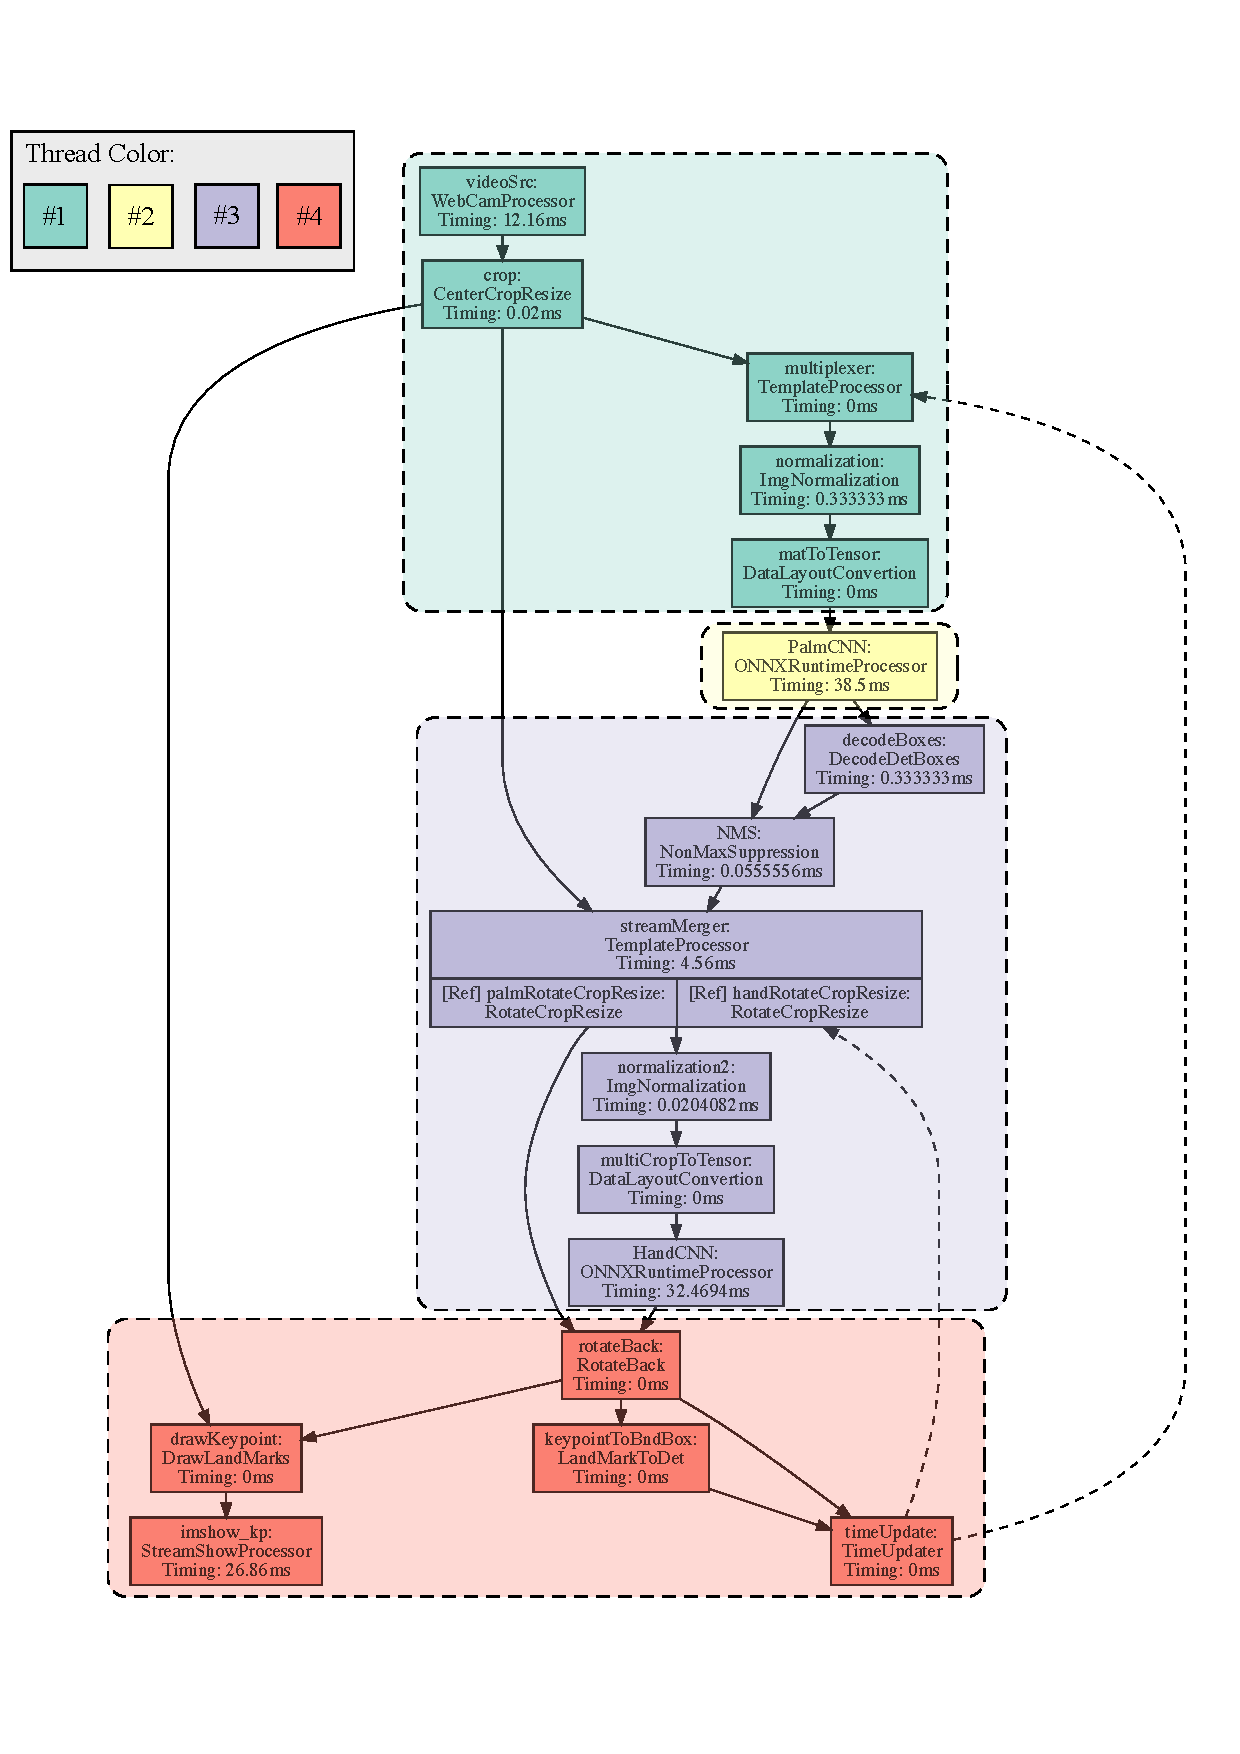
\includegraphics[width=0.7\textwidth]{figure/AVP_multi_hand_tracking.pdf}
    \bicaption[手部追踪任务在AVPipe框架下处理流程的可视化]{手部追踪任务在AVPipe框架下处理流程的可视化。图中虚线连接表示该模块的在本时间戳的输出会在下一时间戳中使用。 由于本图的连接较为复杂,为便于观察,我们没有提供如图\ref{fig:pose_dag}中的Stream可视化,只保留模块间连接。
    节点运行时间信息来自Intel i5-8210Y处理器的MacBook Air的预运行。}{AVPipe visualization of multiple hand tracking video processing task.}
    \label{fig:hand_dag}
\end{figure}

\section{运行环境与参数设置}
目前AVPipe框架完成了对macOS,Linux以及Windows这三大桌面操作系统的支持\footnote{我们会在以后尽可能地提供对移动平台的支持,但这部分并不属于本研究课题所关注的重点。}。同时,由于AVPipe框架的目标设备主要是用户个人的终端,而非高性能的服务器,因此我们选择macOS和Windows这两个主流平台下的便携笔记本电脑作为测试设备(我们手上持有的计算设备也只能支持我们选择这样的测试设备)。对macOS平台,我们使用了一台MacBook Air,其搭载了,
Intel i5-8210Y双核心处理器;对Windows平台,我们使用了一台ThinkPad X1 Carbon,其搭载了Intel i5 10210U四核心处理器。更多核心数量能为多线程运行带来更好的性能,这一点我们也可通过对比这两款设备的处理速度来进行观察。
为体现AVPipe在多硬件场景下的支持,我们还在后续测试中使用了Intel Neural Compute Stick 2(NCS2)\footnote{\url{https://software.intel.com/content/www/us/en/develop/hardware/neural-compute-stick.html}}这一神经网络加速器,以及Intel的核心显卡进行处理流程的构建。\par

在测试过程中,为了尽可能减少其他因素对运行结果的影响,同一处理任务在不同平台下均使用同一视频文件的前200帧作为输入进行分析。在运行视频处理任务时,我们会尽可能关闭系统中其他正在运行的高资源占用进程。我们在这些视频处理任务中所使用的CNN在未特殊说明的情况下均为全精度(float32)模型,且在进行多线程优化时最大线程数量默认为4.

\section{性能对比分析}

图\ref{fig:stats}展示了我们的测试视频处理任务在不同设备上的运行速度。总的来说,我们的测试视频处理任务可以在这些非高性能便携计算设备上达到高于10帧每秒(FPS)的处理速度,这基本可以实现低帧率视频的实时处理。AVPipe提供的多线程优化在对比的各组测试中均可以有效降低视频处理的耗时,下面我们将对此做具体分析。\par

\begin{figure}[htp]
    \centering
    \begin{subfigure}{0.49\textwidth}
    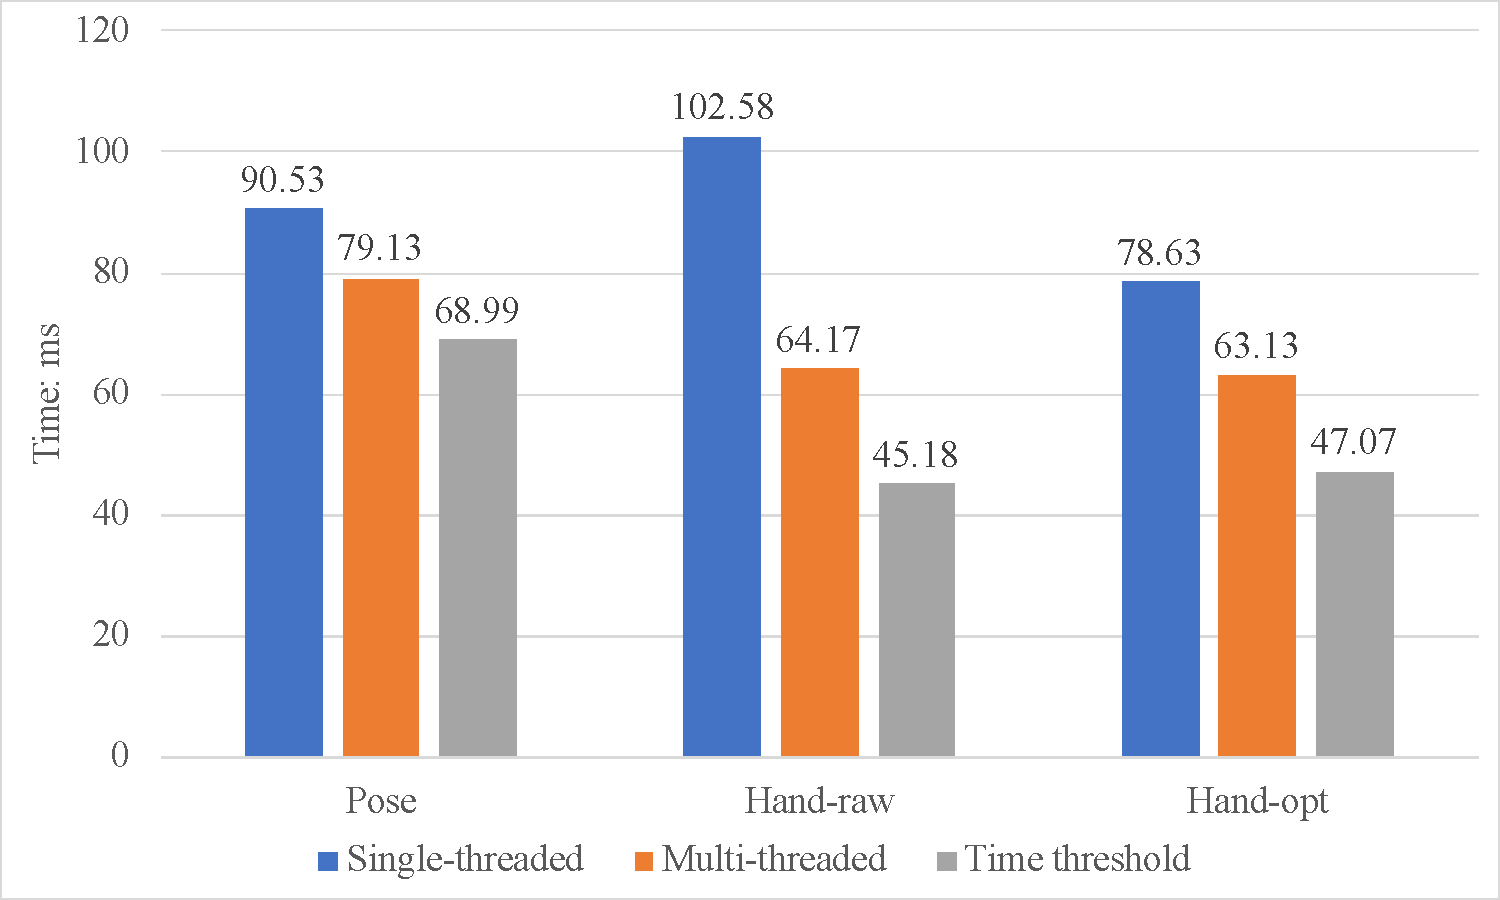
\includegraphics[width=\textwidth]{figure/mac_stats.pdf}
    \caption{MacBook Air, i5 2-Core}
    \end{subfigure}
    \begin{subfigure}{0.49\textwidth}
    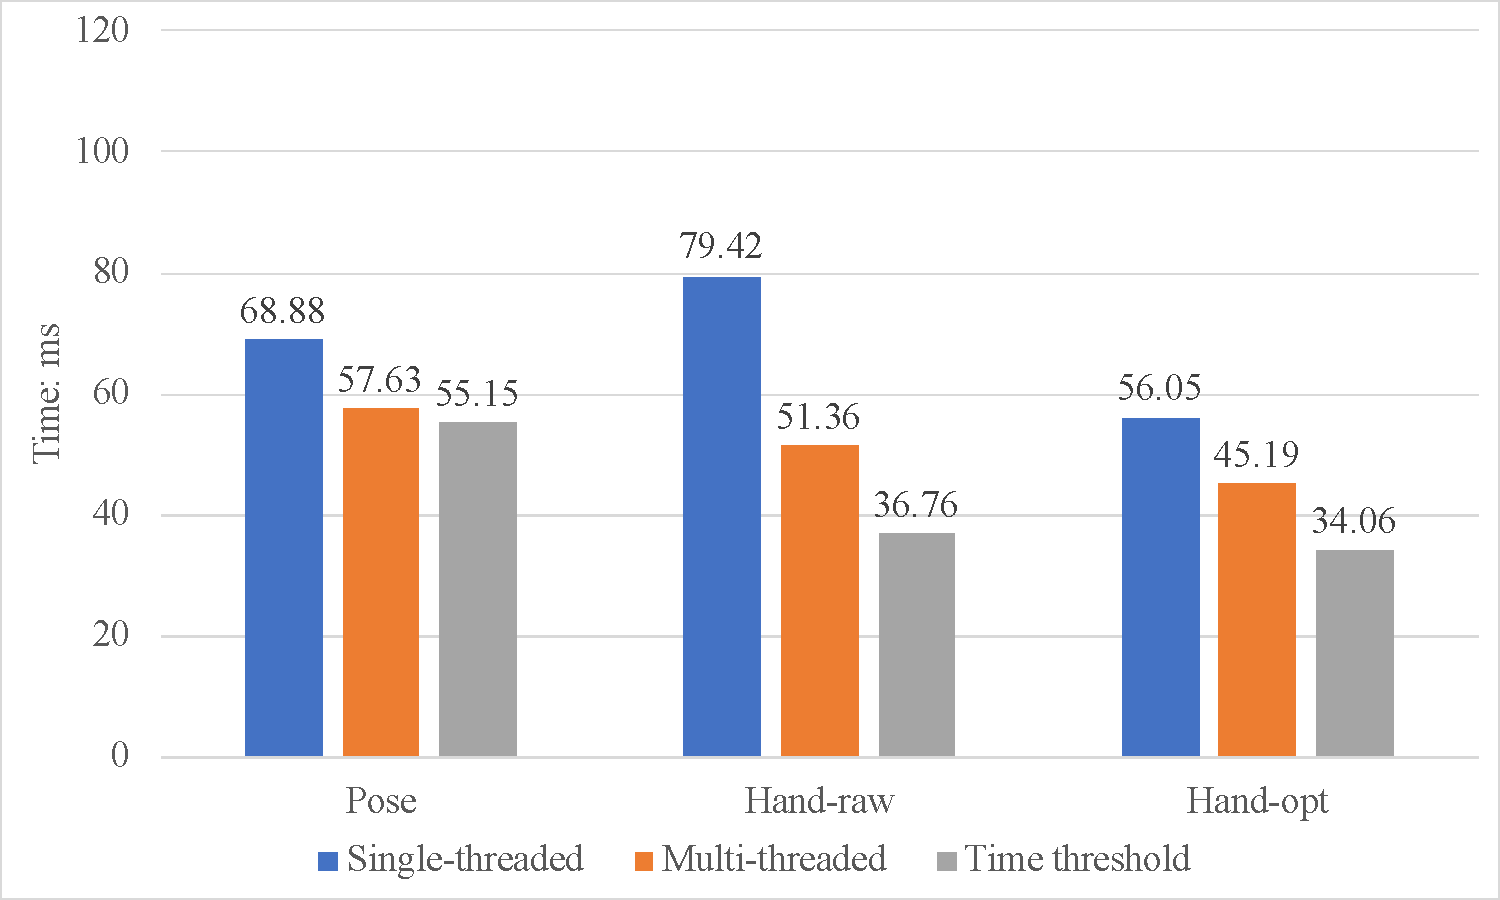
\includegraphics[width=\textwidth]{figure/win_stats.pdf}
    \caption{ThinkPad X1, i5 4-Core}
    \end{subfigure}
    \bicaption[视频处理任务在不同CPU上运行速度测试结果]{视频处理任务在不同CPU上运行速度测试结果,两个计算设备在运行测试任务过程中每帧的平均处理耗时。其中Single-threaded是未优化的单线程运行耗时,Multi-threaded是AVPipe优化后的多线程运行耗时,Time threshold是处理流程中最耗时模块的用时,代表了速度优化的上限。}{Speed testing results on different CPU.}
    \label{fig:stats}
\end{figure}

% 就线程优化程度来说
通过对比经过多线程优化与未经过优化的平均处理时长可以发现,我们的多线程优化策略能够为测试的视频处理任务的平均每帧处理耗时带来超过10ms的提升,这体现了我们所做优化的有效性。在\ref{ch4:autoMT}中我们有提到多线程优化能达到的优化上限是处理流程中最耗时模块的用时(图\ref{fig:stats}中的Time threshold列)。在测试结果中我们可以看到优化后的视频处理任务在耗时上更为接近优化上限,但与理想上限之间仍存在一定的差距。这一差距在具体任务场景下可能是由多种原因造成的,如线程管理上的开销,多线程对计算资源的竞争,流水线各阶段处理速度不同造成的线程阻塞等。
一般来说,越是复杂的处理流程越能通过优化带来更多提升,但越难接近理想优化上限;越是简单的处理流程越能接近理想优化上限,但越难获得较大的优化提升。以图\ref{fig:stats}中的任务为例,Pose任务有更简单的计算流程与模块连接,因此多线程优化空间本身就比较小,较难带来大幅度提升,但是它可以更加接近优化上限,因此Pose任务在ThinkPad上经过优化后基本可以达到与优化上限相同的耗时。
Hand-raw任务在MacBook上经过优化后在速度上有将近40ms的显著提升,但是这一优化结果与理论优化上限相比仍有近20ms的差距。Hand-raw这样的测试结果与其实际数据处理流程有着密切的关系。类似图\ref{fig:hand_dag},Hand-raw在处理每一帧时都会经过两个CNN模型的处理,而这两个CNN模型的耗时又比较接近,因此将这两个高耗时模块放在不同的线程中进行流水线并行优化即可带来较大的性能提升。而Hand-opt由于对处理流程做了算法层面的优化,减少了第一个PalmCNN模型的调用次数,降低了其在单线程上处理的耗时,也缩小了我们进行多线程优化的优化空间。\par

% 就硬件资源来说
从两个平台不同计算资源的对比上来看,拥有更好处理器配置的ThinkPad在各个测试任务中的表现均优于MacBook。从性能优化提升的相对程度上来看,ThinkPad也有着更更好的表现,如图\ref{fig:stats}中两者在Pose任务上的性能优化对比。虽然在Pose任务的优化上两台机器的线程划分均为图\ref{fig:pose_dag}中的形式,存在3个线程,但两台机器在并行运行这三个线程时的额外系统控制开销并不相同。受限于处理器核心数的限制,MacBook只能使用两个核心来分配这三个线程,这必然引入了更多的计算资源竞争,从而无法达到接近优化上限的处理速度。

\section{多线程优化验证}
为了进一步确认AVPipe框架下每个线程的运行情况,同时对优化结果和理论上限之间的差距做合理解释,我们对AVPipe框架下的视频处理任务进行了运行追踪。我们在AVPipe的自动化工具中实现了利用AVPipe框架的运行日志信息(使用了glog\footnote{\url{https://github.com/google/glog}}库)来解析生成各线程的运行时间线(timeline)的脚本代码。运行日志数据会被转换为格式化的json文件,供Google Chrome的Trace-viewer\footnote{\url{http://dev.chromium.org/developers/how-tos/trace-event-profiling-tool}}插件生成可视化的timeline。\par
\begin{figure}[htp]
    \centering
    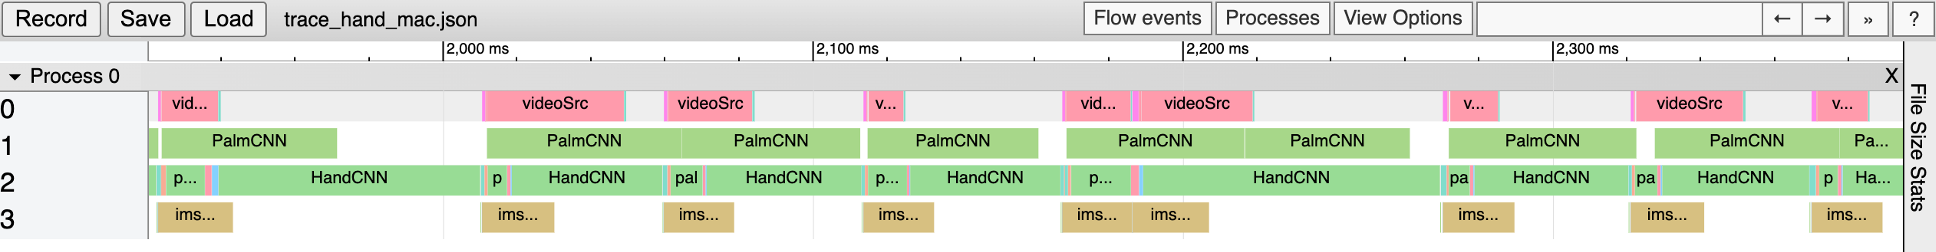
\includegraphics[width=\textwidth]{figure/trace.png}
    \bicaption[AVPipe视频处理任务的多线程时间线]{AVPipe视频处理任务的多线程时间线在Chrome Trace-viewer中的截图。图中不同横行代表不同线程,不同颜色代表不同的处理模块。该流水线是Hand-raw在MacBook上运行得到的。}{The snapshot of AVPipe task runtime timeline in Chrome Trace-viewer}
    \label{fig:trace}
\end{figure}
图\ref{fig:trace}展示了Hand-raw在MacBook上运行时的时间线。从图中可以看到PalmCNN和HandCNN这两个高耗时处理模块被分配到了两个不同的线程中运行。这两个线程也都保持着相对较高的运行负载。从图中所示的这一段运行时间来看,PalmCNN模块存在的断断续续的阻塞是由HandCNN模块无法及时处理掉PalmCNN的结果,导致PalmCNN所连接的Stream容量已满而造成的。由于HandCNN模块的输出是由PalmCNN模块的所有检测结果通过剪裁后获得的,故HandCNN的运行时的batch size是可以变化的\footnote{可以根据实际应用场景将检测数量进行固定,如每次固定只处理batch size为2的输入。},当在一些场景中人手检测数量突然增多时,HandCNN计算耗时会增长,PalmCNN的运行会因数据包堆积而阻塞。这一连串的影响最终导致了我们的优化结果无法达到理论上的优化上限。
尽管如此,高耗时模块的并行计算也确实为整个流程的处理速度带来了明显的提升。

\section{异构计算硬件下的测试}
依靠对不同神经网络推理引擎的整合,AVPipe可以支持使用如GPU,VPU等专用硬件进行深度学习视频处理流程的构建。在本小节中,我们使用Intel GPU与Movidius VPU(NCS2)来代替以上实验中的CPU的来展示AVPipe框架的通用性与可拓展性。
值得注意的是,Intel GPU与NCS2在性能上远不及Nvidia GPU,这两者更关注功耗与便携性,故在实际性能上并没显著优于CPU。但却可以有效降低CPU的资源占用。图\ref{fig:stats_pu}展示了使用VPU和GPU的在各任务上的平均处理时长。可以看到我们的多线程优化同样为各任务的处理效率带来了提升。\par

\begin{figure}[htp]
    \centering
    \begin{subfigure}{0.49\textwidth}
    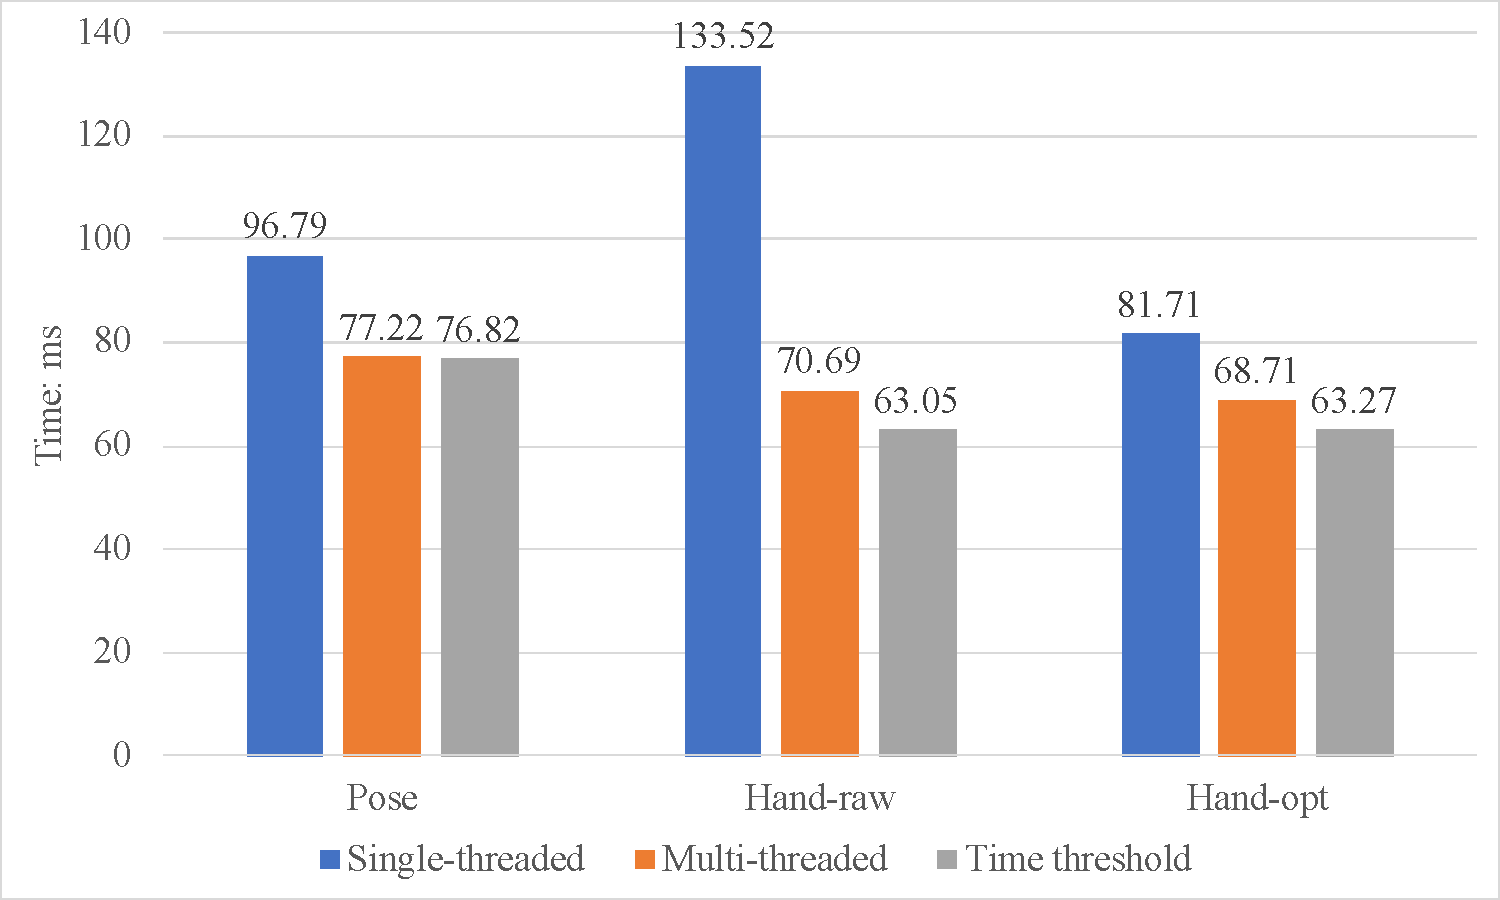
\includegraphics[width=\textwidth]{figure/VPU_stats.pdf}
    \caption{VPU, NCS2}\label{subfig:vpu}
    \end{subfigure}
    \begin{subfigure}{0.49\textwidth}
    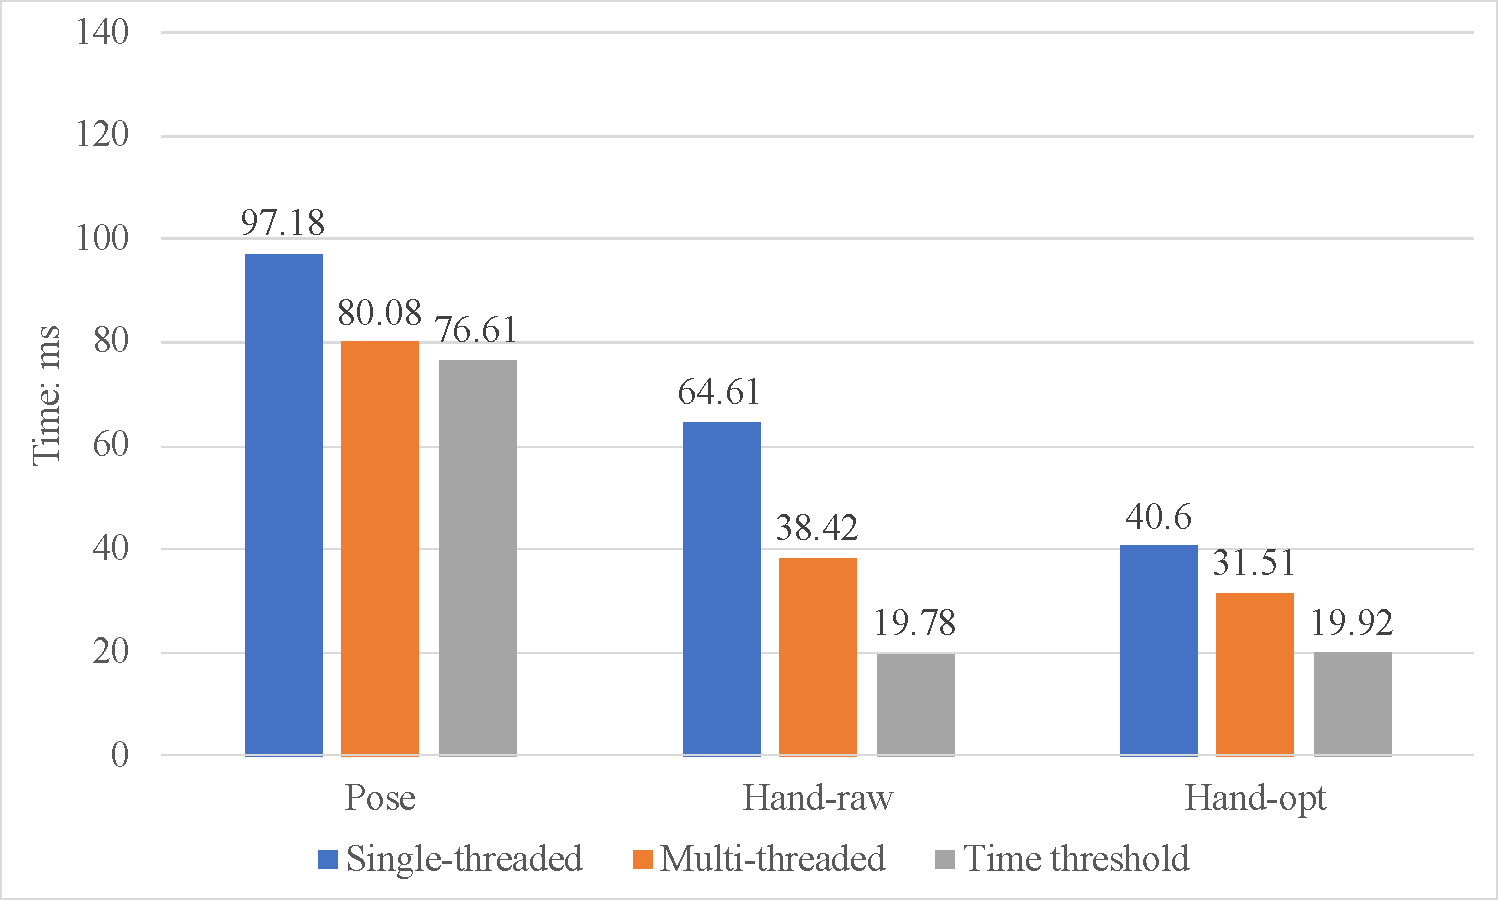
\includegraphics[width=\textwidth]{figure/GPU_stats.pdf}
    \caption{GPU, Intel Iris 540}
    \end{subfigure}
    \bicaption[视频处理任务在不同异构硬件上运行速度测试结果]{视频处理任务在不同异构硬件上运行速度测试结果。由于资源限制,VPU结果中仅PalmCNN模型部署在VPU上,HandCNN在CPU运行;而GPU测试中模型均部署在GPU上。}{Speed testing results on different heterogeneous hardware.}
    \label{fig:stats_pu}\label{subfig:gpu}
\end{figure}

Intel NCS2 VPU主要用途是为低算力的边缘设备(如Raspberry Pi)带来AI算力的提升。由于有这样的设计目标,NCS2本身就属于一个低功耗的微型处理器。因此它在CNN推理上的表现并没有强过桌面级CPU。在图\ref{subfig:vpu}展示的三个测试任务中,VPU上进行的CNN推理均为对应处理流程中最耗时的性能瓶颈模块。由于将大量计算任务分配给了VPU,这使得各线程在对CPU资源的竞争上有所缓解,我们的多线程优化也因此更能够接近VPU推理下的理论优化上限(如图\ref{subfig:vpu}中的Pose和Hand-raw任务)。虽然VPU整体表现上并没有十分突出,但结合我们提供的优化,VPU确实能为一些低算力设备带来实时AI视频流处理的能力。\par
测试视频处理任务在Intel GPU上的表现需要分情况来说明。当推理模型较大较复杂时,如Pose中用到的多路HRNet CNN模型,GPU并不能提供理想的推理加速,其实际推理速度甚至还会略逊于纯CPU的推理速度。但当模型是常规且简单的CNN结构时,如Hand任务中的PalmCNN和HandCNN,GPU是能够在模型推理上带来较大幅度性能提升的。这也使得经过处理算法和系统多线程优化后的Hand-opt可以达到30FPS以上的实时处理速度。在另一方面,由于Hand任务中两个CNN模型均部署在了GPU上,当多线程调用GPU进行模型推理时,必然会存在一定程度的计算资源竞争,因此我们的多线程优化很难达到单一模型速度所代表理论优化上限。

\section{本章小结}
在本章中,我们展示了几个实际视频流处理任务在AVPipe框架下的实现。然后以这些任务为例进行AVPipe的多线程优化的测试。测试视频处理任务在各个情况下均有提升的结果说明了我们提供的多线程优化策略的有效性与通用性。接下来我们又对AVPipe框架下的多线程处理任务的实际运行情况进行追踪,对AVPipe多线程优化所能带来的性能提升程度做了合理的分析与解释。最后,我们展示了AVPipe测试任务在其他异构硬件上的运行效果,由此来说明AVPipe框架的高拓展性。通过不断地进行算法层面与系统层面的优化,我们相信AVPipe在以后还能为AI视频处理任务带来更多的加速。
% !TEX root = ../thesis.tex

\begin{summary}
本研究课题针对深度学习背景下的视频流处理任务提出了Aceel-Video Pipe(AVPipe)这一C++编程框架,为视频流处理任务提供开发流程与处理速度上的优化。\par
在开发流程上,我们通过对各类视频处理任务进行分析与总结,将整个视频处理任务抽象为数据包(StreamPacket),数据流(Stream),数据处理单元(PipeProcessor)这三者的互联与组合。为此,我们进行了C++相应代码的实现。在实现过程中,我们对处理流程可能涉及的数据类型、数据格式进行了统一与整合;对数据的多线程使用提供了必要的同步与阻塞机制;对多种深度学习推理引擎与计算硬件提供了支持,并简化和统一了调用接口。除了提供较完善的C++库的定义与实现,我们还进一步为便利开发提供了自动化工具。
通过定义处理流程的配置文件,AVpipe可实现自动化的C++代码生成,任务处理流程可视化以及处理流程运行时追踪与分析。\par

在处理速度上,我们为AVPipe提供了针对视频处理任务的多线程优化工具。通过视频处理任务运行时的性能分析,我们可以获得整个处理任务中每一模块的计算用时。多线程优化工具依据这些信息,利用视频处理流程存在的DAG计算模式与流水线计算模式, 将高耗时的瓶颈计算模块划分在不同的线程以实现数据处理的并行化计算。在多线程优化工具的具体实现上,我们提出了有针对视频处理任务特点的启发式DAG处理流程划分算法,在尽可能多线程平摊计算任务的同时,保证多阶段流水线的数据上下依赖关系。\par

最后,通过对一些具体视频处理任务的实现,我们展示了AVPipe的开发流程与性能优化。测试结果表明了我们提出的多线程优化策略的有效性,在某些情境下AVPipe的多线程优化可以提供将近一倍的速度提升。我们之后在GPU与VPU上的测试也进一步展现了AVPipe框架的通用性。\par

AVPipe将会作为一个开源项目在未来继续进行框架的优化与改进。我们会为其持续添加新的计算模块与开发文档;提供可视化的流程连接与参数配置的前端操作界面;移动平台的完善支持;更细粒度的针对视频处理任务的算法与系统层级的优化。我们十分期望AVPipe未来能够在实际生产开发中展现其应有的使用价值。
\end{summary}

% 使用英文字母对附录编号
\appendix

% 附录内容,本科学位论文可以用翻译的文献替代。
% \input{tex/app_maxwell_equations}

% 文后无编号部分
\backmatter

% 参考资料
\printbibliography[heading=bibintoc]

% 用于盲审的论文需隐去致谢、发表论文、参与项目、申请专利、简历

% 致谢
% !TEX root = ../thesis.tex

%TC:ignore

\begin{acknowledgements}
\begin{itemize}

\item 感谢冷静文老师对本研究课题的认可与支持!由于毕设的最初研究课题并非“视频流处理优化”,在之后与冷老师沟通,根据个人实际情况在更换为“视频流处理优化”这一课题,没有老师的通融与理解,就不会有如今的毕设论文。其次还要感谢冷静文老师对本项目提供的宝贵指导与意见!这对本毕设的合理开展提供了很大帮助。
  
\item 感谢姚顺宇学长及其创业公司我咖科技团队对本项目的大力支持!选择本课题的很大程度是受学长智能视频应用相关创业项目的影响而选择的。本论文中的测试部分所使用的视频处理任务的CNN模型文件都是由姚学长的团队提供的。我也十分相信的AVPipe框架会在公司今后的视频应用开发上进行实际应用。
  
\item 感谢上海交大学生训练中提供的Nvidia GPU以及Intel Neural Computing Stick 2为本课题带来多样的异构计算资源!
  
\item 感谢所有给予我帮助与鼓励的家人,老师与同学,你们的祝愿是我持续向前的动力!
  
\item 感谢各个图书馆,自习室为我提供的安静且安全的学习环境,尤其是在今年全球疫情这样特殊的情况下,更应值得感激!

\item 感谢 \LaTeX 和 \href{https://github.com/sjtug/SJTUThesis}{\sjtuthesis},为本文排版带来的巨大帮助。

\end{itemize}
\end{acknowledgements}

%TC:endignore


% 发表论文、参与项目、申请专利、简历
% 盲审论文中,发表学术论文及参与科研情况等仅以第几作者注明即可,不要出现作者或他人姓名
% \input{tex/publications}
% \input{tex/projects}
% \input{tex/patents}
% \input{tex/resume}

% 中文学士学位论文要求在最后有一个英文大摘要,单独编页码,英文学士学位论文不需要
% !TEX root = ../thesis.tex

\begin{bigabstract}
Artificial Intelligence is absolutely one of the most popular topics in the area of computer science. Recent years have witnessed the fast development of AI-related technologies, especially deep learning technology. Due to its strong feature representation ability, deep learning has gained great success in many important domains such as computer vision, natural language processing and speech recognition, of which computer vision (CV) is the most successful one using deep learning. By using convolutional neural networks (CNNs), deep learning method has achieved great performance in many visual perception challenges including classification, object detection, pose estimation, etc. Thus, deep learning-based computer vision technology is now widely used in production, which can provide convenience to the industry and our daily life. Intelligent video perception is one of the important categories and forms of deep learning-based CV production application. Basically, video perception can be treated as a fixed workflow that continuously processes a specific CV algorithm frame by frame in the video stream. These intelligent video perception tasks are very helpful not only for other advanced AI applications such as autonomous driving and intelligent robotics but also for providing a greater experience for user content creation. 

Though intelligent video stream processing can bring many benefits in real applications, it is relatively difficult to build such video processing pipelines and run it efficiently in users' general computing devices. Firstly, deep learning related video processing tasks usually have complicated processing pipelines containing multiple processing stages related to operations on visual images or high-dimensional tensors. To deploy such pipelines using programming language like C/C++,  you have to write hundreds of or thousands of lines of code, which is pretty hard for those developers without much background knowledge.

Secondly, deep learning, i.e., neural network models usually contain lots of matrix computation which results in more computational resources consumption and more processing time compared to traditional CV methods. Given such characteristics of neural network models, many dedicated software libraries and hardware accelerators are proposed to optimize and accelerate the NN inference process. When we build some video processing pipeline for real-time processing, we may need to select some optimized libraries or hardware for speeding up, which further increases the cost of development.

In order to simplify the development workflow and to optimize the processing speed for intelligent video stream processing tasks, we propose Accel-Video Pipe (AVPipe),  a C++ programming framework aiming to provide better development experience and runtime performance for video stream processing tasks.

Generally, there are 4 strategies to optimize video stream processing tasks, which are: (a) system-level optimization for the overall video processing workflow, e.g. making use of thread parallelism of dependency-free nodes in processing DAG (Directed Acyclic Graph) or multi-stage processing pipeline;  (b) algorithm-level optimization for the overall video processing workflow, e.g. the continuity of visual motion inside consecutive video frames can be used to propagate processing output of one frame to the next frame thus avoid redundant visual computing; (c) processing component level optimization for video processing workflow, especially the optimization for neural network inference component, e.g. model compression, model pruning, model quantization, etc.; (d) hardware-level optimization for video processing workflow, e.g. there are various dedicated neural computing acceleration chips like GPU, TPU, VPU, etc. In order to do some generalized optimizations for a random video stream processing task implemented in AVPipe, we have to choose system-level optimization as our main optimization strategy. Meanwhile, the other strategies are also supported when doing task-related optimization in AVPipe.

To simplify the development workflow, we do a survey on different kinds of video processing tasks to analyze and summarize some common features for the purpose of framework-level data structure abstraction. In our framework, the whole video processing workflow can be treated as a complex combination of 3 basic structures of AVPipe, which are StreamPacket, Stream and PipeProcessor respectively. StreamPacket contains the raw data to be processed; Stream connects different PipeProcessors and directs StreamPacket to its own consumer; PipeProcessor does the actual data processing. To implement these structures in AVPipe, we give special consideration to (a) the integration of different data types and different data formats (e.g. uint8 Mat, float16 Tensor) in StreamPacket structure; (b) necessary thread synchronization and blocking mechanisms to guarantee the data timestamp consistency and avoid race conditions; (c) support for various neural network inference engines and related  computing devices to give simple and unified interface for all libraries of the same function. 

To simplify the development workflow, we do a survey on different kinds of video processing tasks to analyze and summarize some common features for the purpose of framework-level data structure abstraction. In our framework, the whole video processing workflow can be treated as a complex combination of 3 basic structures of AVPipe, which are StreamPacket, Stream and PipeProcessor respectively. StreamPacket contains the raw data to be processed; Stream connects different PipeProcessors and directs StreamPacket to its own consumer; PipeProcessor does the actual data processing. To implement these structures in AVPipe, we give special consideration to (a) the integration of different data types and different data formats (e.g. uint8 Mat, float16 Tensor) in StreamPacket structure; (b) necessary thread synchronization and blocking mechanisms to guarantee the data timestamp consistency and avoid race conditions; (c) support for various neural network inference engines and related computing devices to give a simple and unified interface for all libraries of the same function. 

In addition to the basic definition and implementation of C++ libraries, we provide some automation tools for the further simplification of development. We add an auto code generator to generate the C++ code of a video processing task according to the YAML configuration file formatted by us. Using such configuration files, we can also plot the DAG of the corresponding video processing task. Moreover, a performance profiling tool is implemented to do tracing and timing of different computing component of the whole video processing graph.

To optimize the performance of video processing tasks implemented by our AVPipe, we implement an auto multi-threading optimization tool. There two typical parallelism patterns inside these video processing tasks: parallelism of dependency-free nodes in DAG and parallelism of the multi-stage pipeline with one-sided dependency.  Following these two patterns, our multi-threading optimization tool takes use of tasks' runtime profiling information to filter out some high time-consuming PipeProcessors (i.e., bottleneck processing components) from the video processing graph, and try to make these bottleneck processing components to be placed in separated threads so that some processing time can be overlapped thus processing speed will be improved. When it comes to the actual implementation of our optimization, we propose a heuristic DAG partitioning algorithm to exploit the parallelism patterns mentioned above. In this algorithm, we iteratively put high time-consuming processing components into new threads and do necessary component merging based on the local dependency of these components. There is a theoretic upper bound for our optimization which is the time used by the most time-consuming component, but we may not reach this upper bound for many reasons including the limitation on the number of threads, computation resource contention, complex dependencies among different threads, etc.

We then showcase two video stream processing examples and testify the effectiveness of our multi-threading optimization. The two video processing tasks are pose estimation task and multi-hand tracking task. To show the flexibility of our framework, we also do some CV algorithm level optimization to multi-hand tracking task by adding some user-defined computing components and asynchronous Stream connections. Our test results show that our multi-thread optimization can bring performance improvements for all test cases on different devices including CPU, GPU and VPU. The scale of improvements depends on the complexity of the processing tasks. In some cases, our optimization can even provide almost 1x speedup compared to the corresponding vanilla processing tasks. These promising results prove our AVPipe framework's high effectiveness and high extendability.

As an open-source programming framework, AVPipe will keep adding new functions and improving its supports in the future. We really hope our AVPipe framework will play an important role in the future development of video stream processing applications.

\end{bigabstract}


\end{document}
